\section{Anthony K Tigerius III}

\begin{center}
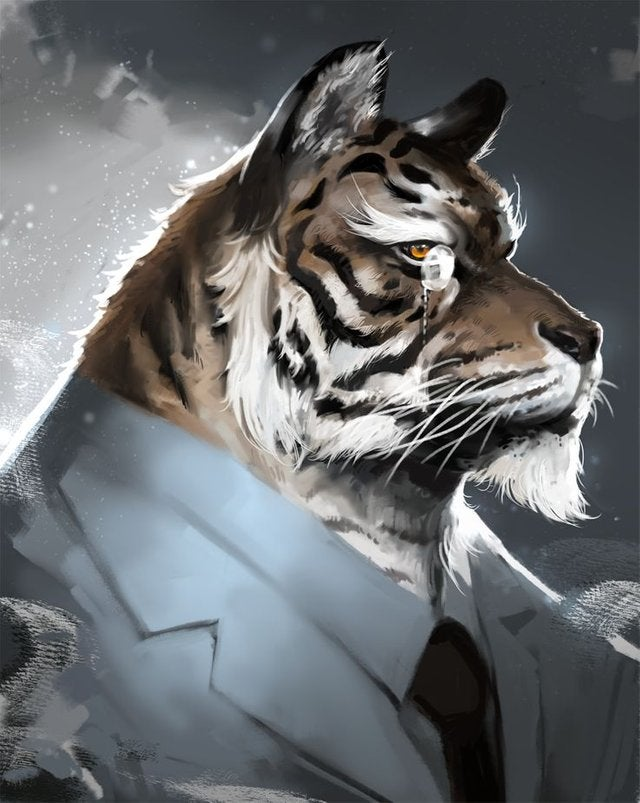
\includegraphics[width=80mm]{./content/img/toniTiger.jpg}
\begin{figure}[h]
\end{figure}
\end{center}

\subsection*{Details}

\noindent

Race: 	DesertCat \\
Class: 	Barbarian \\
Age: 	42 \\
Status: Wandering the Expanse (assassin contract if he returns)

\subsubsection{Background}

Anthony K. Tigerius III arrived at the party's airship by Hope's Restian stagecoach, stepping out as a large, well-dressed tiger carrying a briefcase and holding a cane he clearly did not need.  Sent by the Guild of Coin to open negotiations regarding Riphard Obsidian Hardstone's considerable fortune, he found instead a group of fugitives, a petrified dwarf, and a pregnant Jenny.

His formal correspondence with the Guild, fragments of which survived the flooding of a records office in the Age of Abject Terrors, reveals a methodical mind struggling to reconcile the group's obvious insanity with their equally obvious capability.  He followed them into the Tom'ardy mines on the justification that if the tales about the airship were true, then perhaps the group really was ``as capable and insane as they say.''

\subsubsection{Personality and Traits}

Toni was the group's most professional member, a trained negotiator and diplomat who believed in structure, synergy, and the proper use of breakout rooms.  He set up a powerpoint presentation to train Lady Gharbighast's staff in negotiation tactics, used the word ``synergy'' to clinch deals with fish kings, and maintained formal letters to the Guild of Coin even as the world fell apart around him.

Beneath this veneer of corporate civility, however, lurked a primal berserker fury.  When sufficiently ``peeved about the injustice of it all,'' the mild-mannered Anthony bit his lip, spat blood, and gave way to a blur of cane-sword and rage.  His berserker state first manifested in the deep mines, where he single-handedly saved Burnie from a four-armed horned abomination by pounding its exterior in a frenzy, then ran off to attempt to murder a dwarf that had been dead for hundreds of years.  He later apologised to Exme for acting ``so uncouthly.''

He fed his companion starlings by hand on the deck of the airship, and they sang little songs to each other which was very nice.

\subsubsection{Relationships}

Toni saw Riphard as an un-tempered prodigy who could take the world by storm.  His hope was that the power and wealth Riphard wielded could be directed toward the betterment of all Velterra, and his negotiations with the Guild of Coin were motivated by this larger vision.

He provided a calming counterbalance to Burnie, once pulling him aside to politely explain ``why he was wrong about almost everything'' during the merfolk negotiations.  His exchanges with Exme were warm, she showed him her ``dinglehopper,'' and he gave her ritual materials to talk to animals that she built into her helmet.

Toni's relationships with the wider group were defined by a growing moral unease.  He saw the party commit acts of terrible violence, some under magical ensorcellment and some by choice, and it weighed on him.

\subsubsection{Toni's Story}

Toni joined the party during the expedition to the Tom'ardy mines, where his berserker rage saved Burnie's life in the battle against a creature that ``should definitely not exist.''  He accompanied the group through the deep mines as they searched for Excalibrum, though his formal Guild of Coin dispatches struggled to convey the increasingly bizarre reality of the situation.

His finest hour came at New Abbergast, where the party had been tasked with resolving a conflict between the land settlers and the merfolk who were attacking their fishing boats.  Toni personally captured a merfolk warrior, negotiated a diplomatic meeting with King Oceani of the Waves, trained Lady Gharbighast's staff in negotiation tactics via powerpoint, and brokered a trade agreement that resolved the conflict peacefully, one of the few problems the group ever solved without significant bloodshed.

The breaking point came at Golding's Bay.  A temple's magical ensorcellment caused the party to slaughter an entire village of innocent people.  Toni was disgusted.  When the Arbiters arrived to investigate, he walked out of the church, stated his name and cause, and dropped to his knees in surrender, the only member of the group to willingly face justice.  Arbiter Kiros used a word of truth on him, and under its influence he confessed to the crimes, despite having been ensorcelled at the time.  He was beaten, battered, and dragged away to a prison wagon.

Burnie rescued him through an audacious deception, but the damage was done.  From the crow's nest of the airship, alone with his thoughts and his remaining starlings, the tiger looked aloft and thought: ``They are monsters, they are foul debasers, they shall pay for what they have wrought.''

Toni left the group in the night, heading toward the Expanse to find his family.  The party, characteristically, hired assassins to kill him if he ever returned.


\begin{center}
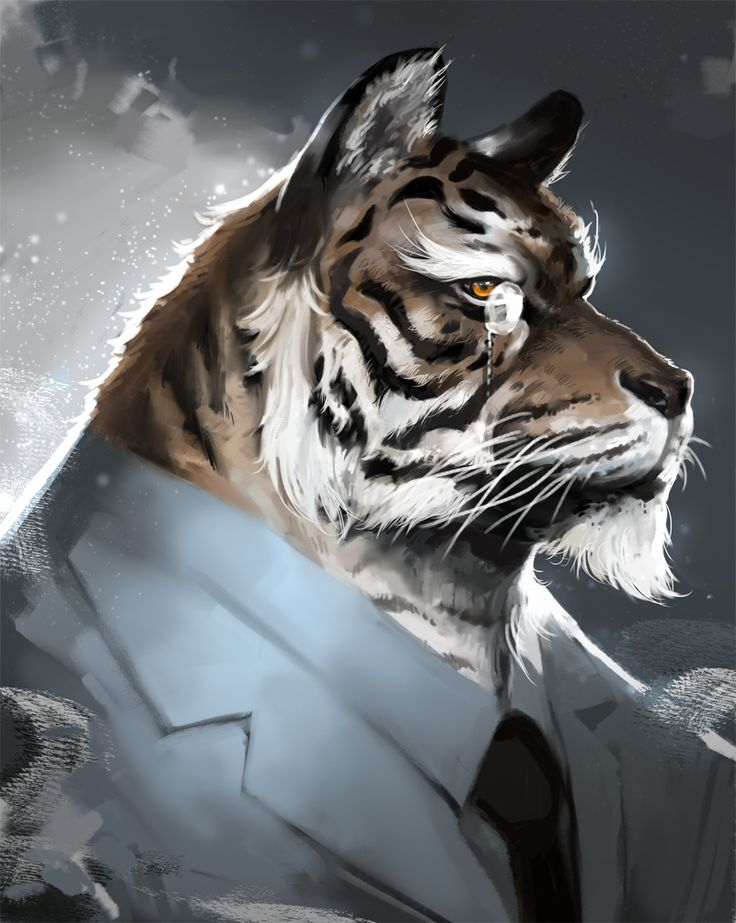
\includegraphics[width=80mm]{./content/img/reddit/anthonyTigerius.jpg}\\
\textit{Anthony K Tigerius III}
\end{center}

\clearpage
